\section{Chemical Cloud Detection with UAV Swarms}

In order to further test the simulation capabilities of \SWEEP{}, a real-world problem was selected for simulation and modeling within \SWEEP{}.  The scenario chosen involves unmanned air vehicles attempting to coordinate in order to detect a chemical cloud.

\subsection{Introduction}

Swarm algorithms can coordinate UAVs in situations that require a level of flexibility and robustness unattainable by a single, more complex air vehicle controller.  Additionally, achieving effective use of UAVs requires more than just controlling a single vehicle; the larger problem, with a potentially greater payoff, resides in establishing coordinated behavior of many such vehicles \cite{clough:SwarmingUAVs}. While much work has been done applying emergent behavior and swarms to a wide variety of problems \cite{palmer:Behavior, bonabeau:SwarmSmarts, lewis:Nanorobots, balch:FormationControl, orbital:SatelliteSwarms, go:AutonomousBehaviors}, there has been a deficiency in simulating realistic air vehicles within swarms. Air vehicles have been modeled as particles \cite{trahan:UAVSwarms}, as objects that can arbitrarily move within a hexagonal grid \cite{parunak:DigitalPheromone} or as detailed \textit{individual} representations of actual aircraft \cite{isreal:PredatorModeling}.  This simulation considers both issues: \textit{swarms} of air vehicles that \textit{respect the physical realities of their flight envelopes}. The model of the flight envelope is both general enough and realistic enough to apply to a wide variety of UAVs.  Also, an equivalent of randomized motion within motion constraints is defined and is used to build simulations of UAV missions that exhibit emergent behavior.

The main simulation scenario used in the development and evaluation of UAV swarm control strategies was that of a chemical cloud threat, as shown in \refFigure{Scenario}. In this scenario, a UAV swarm is assigned a region to patrol, with the objective being to determine if a chemical cloud is present. The swarm is deployed from a tower-like structure, which could include the roof of a tall building. Once deployed, the UAV swarm executes various distributed search algorithms. If a cloud is detected, many actions can be taken, such as attempting to map the size and density of the cloud. Also, if a UAV does find the cloud, and subsequently becomes contaminated, it must not return to the home base, but to a predefined decontamination center.

\begin{figure}[ht]
  \centering
  %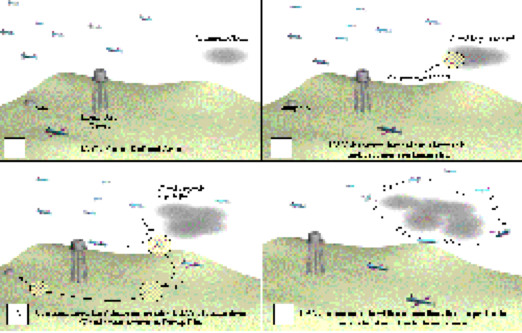
\includegraphics[scale=2]{Figures/Scenario.pdf}
  \begin{minipage}{\linewidth}
    \subfigure[Deployment]{\fbox{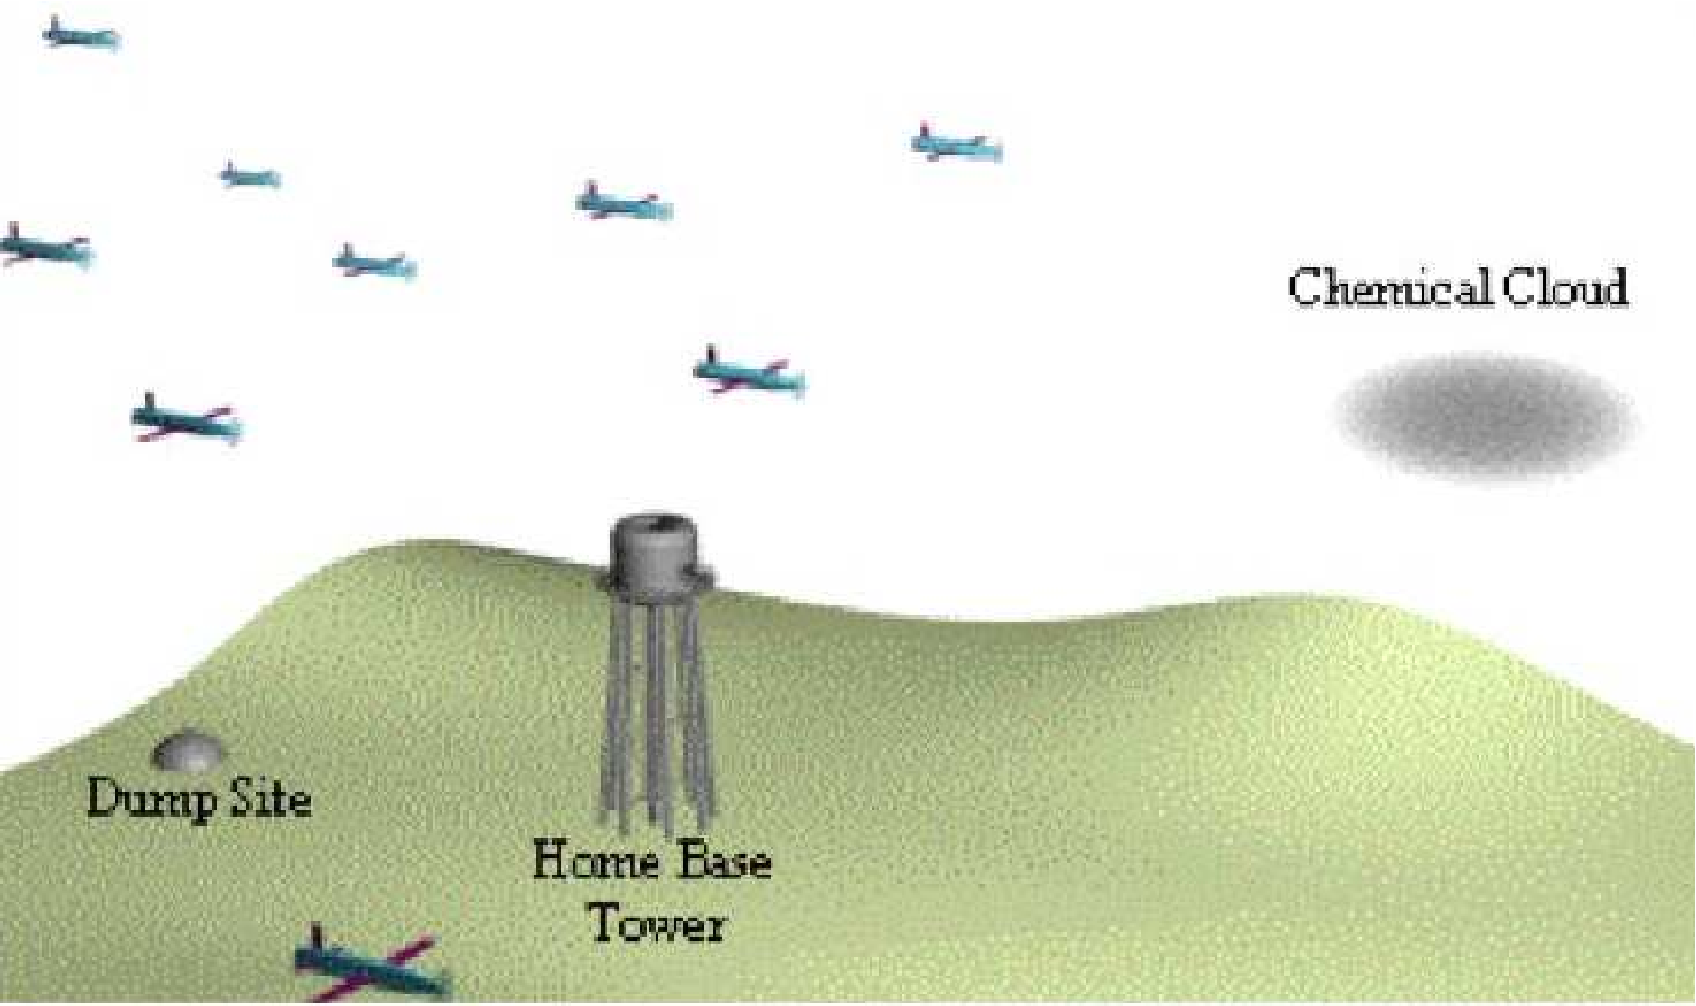
\includegraphics[width=.4\textwidth]{CloudScenario-1}}}
    \qquad
    \subfigure[Detection]{\fbox{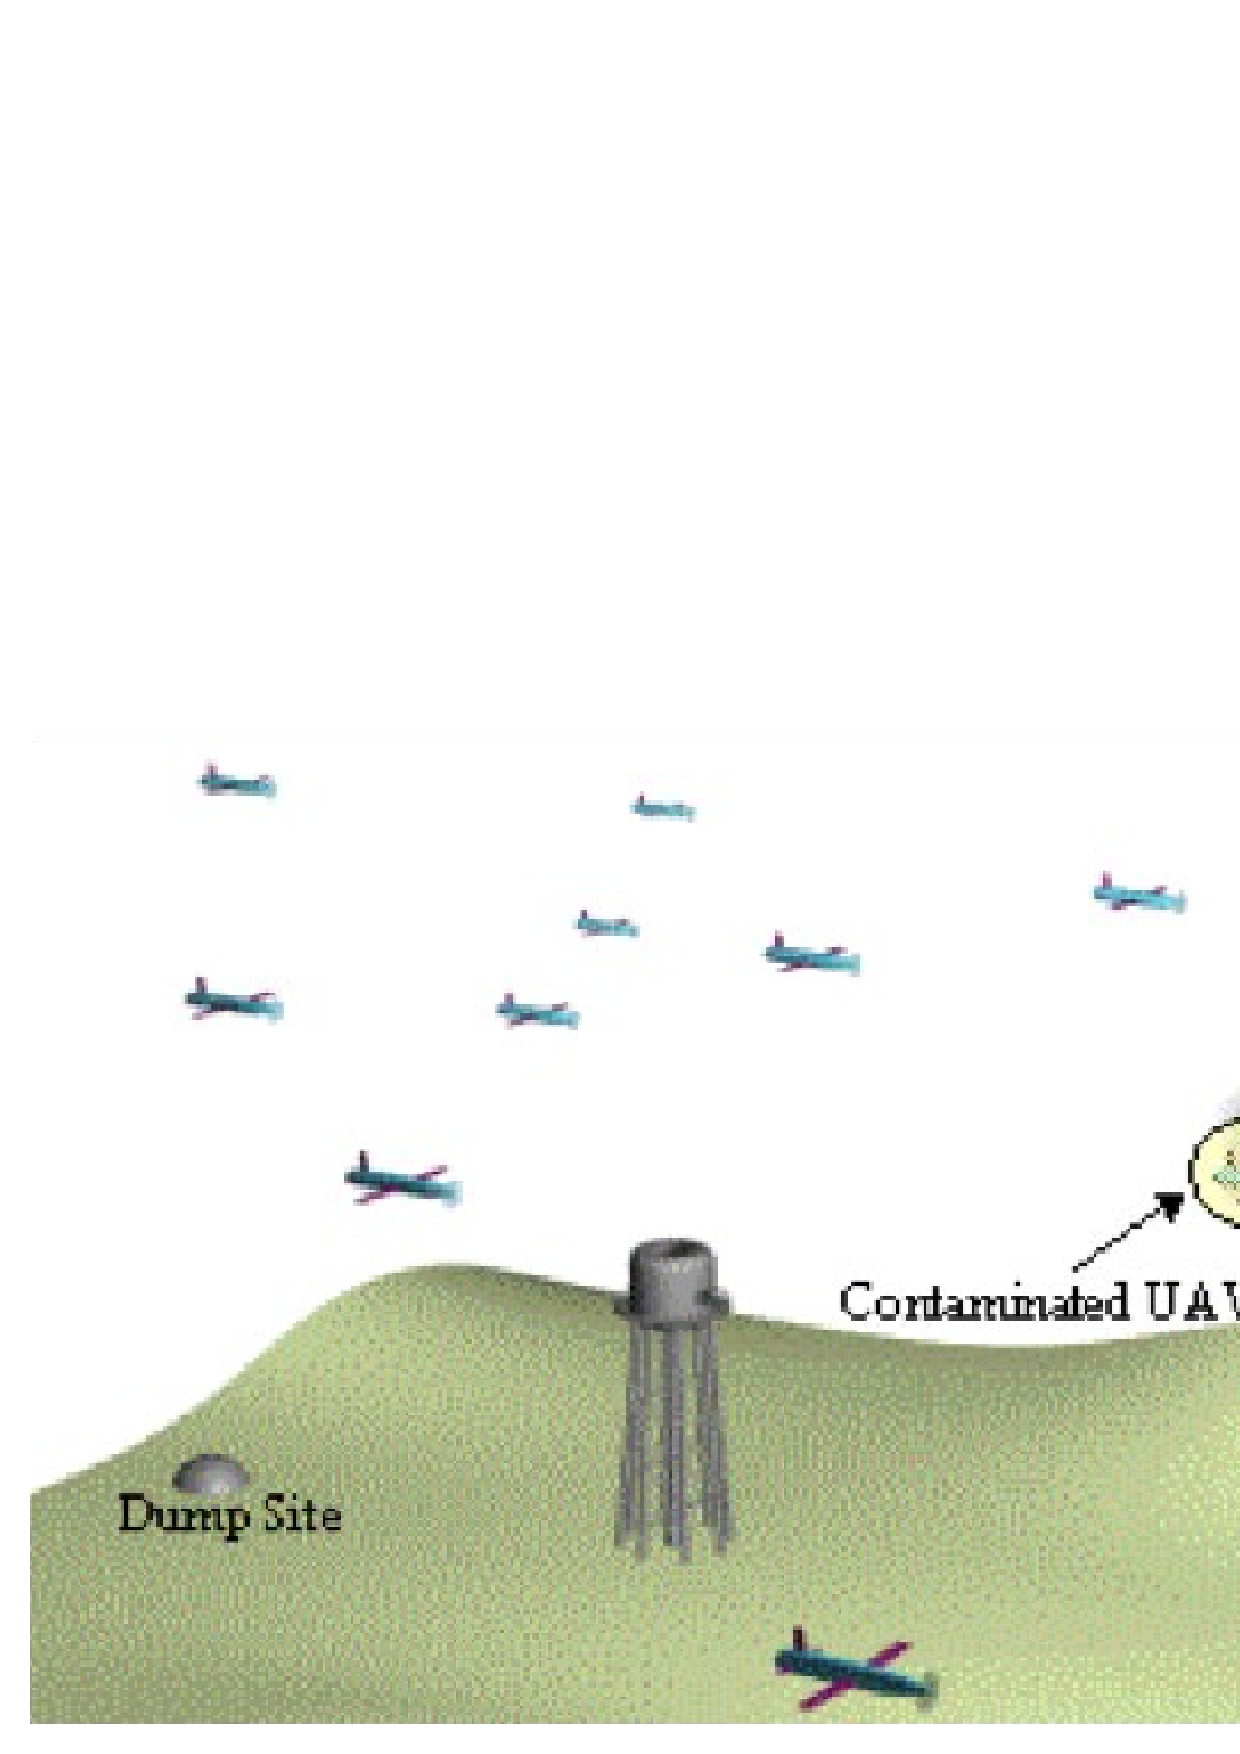
\includegraphics[width=.4\textwidth]{CloudScenario-2}}}
    \centering
    \subfigure[Mapping]{\fbox{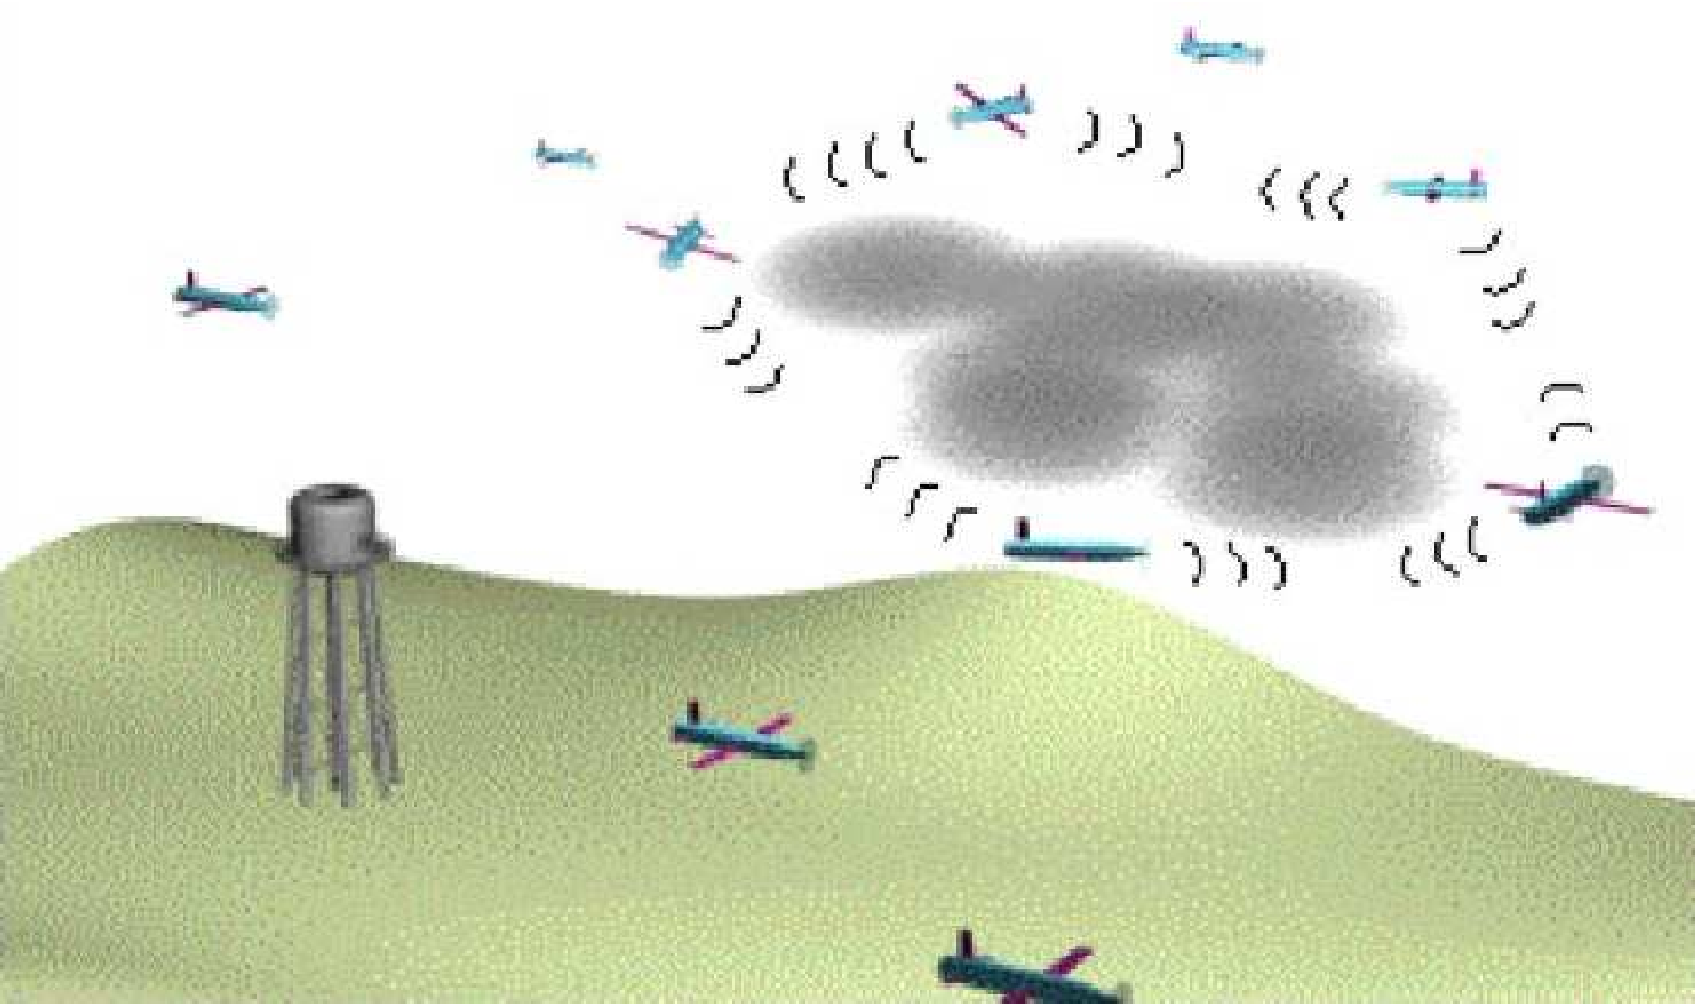
\includegraphics[width=.4\textwidth]{CloudScenario-3}}}
  \end{minipage}
\caption{The different stages of a chemical cloud detection mission: deployment, detection, and mapping.}
\label{fig:Scenario}
\end{figure}

\subsection{System Overview}

In order to aid the development and simulation of emergent behavior strategies for UAVs, an optimal path planner that respects the UAV flight envelope is used. The optimal path planner uses simple geometric operations to construct the optimal flight path between two points for a UAV traveling at a constant speed. Given the destination and desired final heading, the optimal path planner constructs a control history for the UAV \cite{yang:PathPlanning}. 

\paragraph{Postulated UAV Configuration}

Swarm intelligence algorithms focus primarily on emerging complex behaviors from simple agents. With this in mind, the postulated UAVs are as minimalist as possible, thus allowing the developed strategies to be applicable over a broad range of UAVs. The developed algorithms can be easily built upon to leverage the capabilities of more advanced UAVs. 

The UAVs are assumed to have a constant velocity of 40 knots. Computing capabilities will be comparable to a 66 MHz computer. Some form of inter-agent communication is assumed to be present, with no bias towards global communication capabilities. The UAVs will have modular sensor arrays that can accommodate specific mission requirements. The battery or fuel cell for the UAVs should provide at least one hour of operational time and be able to be recharged while detached from the craft.

In this 2D model (\refFigure{FlightModel}), the UAV is a point mass with its state specified by $(x,y,\theta )$, where $(x,y)$ is the instantaneous position and $\theta $ is the heading angle. In addition, $\omega $, which is the time rate of change of heading angle, is a controllable input. It is assumed that the input $\omega $ is bounded by $[-\Omega ,\Omega ]$. Such bounds for the control input are due to the limits on the flight envelope of UAV turning rate and speed. As per the postulated UAV configuration, a constant velocity $v_C$ is assumed.

\begin{figure}[ht]
  \centering
  $\left\{ 
  \begin{array}{l}
    \dot {x}=v_C \cos (\theta ) \\ 
    \dot {y}=v_C \sin (\theta ) \\ 
    \dot {\theta}=\omega \\
  \end{array}
  \right.$
\caption{Postulated UAV flight model}
\label{fig:FlightModel}
\end{figure}

\subsection{Search Algorithms}

UAV swarms are well-suited for tasks involving reconnaissance due to their inherent parallelism and highly robust nature. A monolithic air reconnaissance platform can only observe a single area at a time, and no information can be obtained if the aircraft is disabled. These restrictions do not apply to UAV swarms. The parallel nature of a UAV swarm can allow multiple areas to be observed by a single swarm, but also allows for continued reconnaissance even if multiple members of the swarm are disabled.

\paragraph{Restrictions\\} The largest obstacle encountered when designing search strategies for UAV swarms is managing the physical restrictions of the UAV. There are four main restrictions when it comes to UAV performance: flight envelope, radar and communication, on-board processing power, and fuel supply. 

The flight envelope of a UAV is very restrictive. The cruising speed and turning radius of the UAV are such that even the most basic search strategies need to account for these factors. For example, if the objective is to locate or track a fast moving object, the total area being simultaneously searched may have to be reduced in order to improve the overall accuracy of the swarm due to the low cruising speed of the individual UAVs.

Typically, in reducing the power, size, and cost of a UAV, the communication and radar capabilities of the UAV are comparably diminished. These restrictions greatly impact emergent behavior search strategies attempting to magnify the capabilities of the swarm. For example, a swarm of UAVs with low-resolution sensor footprints could locate an object smaller than their sensor footprint by merging their individual sensor readings while still only requiring minimal communication overhead \cite{clough:SwarmingUAVs}.

Search strategies for UAV swarms must expect limited on-board computation capabilities, thus complex calculations will be either too slow or impossible to perform in a real-time environment. Therefore, highly computational search strategies will not be very effective.

Perhaps the most severe restriction is battery life. If a UAV can only be operational for one hour before its power supply is completely drained, then one knows how sufficiently efficient and reliable a search strategy must be. 

\subsubsection{Randomized Search} Randomized searching is the most basic search strategy capable of being implemented on a UAV swarm. Each UAV chooses a random heading and a random amount of time, and then proceeds to fly in that direction for that duration. The operational requirements for randomized searching are minimal. No communication capabilities need be present on-board the UAV. The randomized search is adaptable for any type of flight envelope and sensor array. As can be expected from any distributed, randomized algorithm, results can only be guaranteed in a probabilistic manner. When the number of UAVs is low, emergent behavioral algorithms suffer and perform no better than any other strategy. 

\subsubsection{Symmetric Sub-region Search} A symmetric sub-region search divides the search area into equally shaped and sized regions, assigning one or more agents to each region. For example in \refFigure{SymmetricSearch-1}, eight circular subregions are defined around the perimeter of a known safe-zone.  In this scenario, the goal is to be able to detect when a threat incurs through the perimeter.  In \refFigure{SymmetricSearch-2}, no information is known about the region, so it is equally probable that a threat can occur anywhere.  Thus, the entire region is subdivided into equally sized units of which a subset will be assigned to a each UAV to patrol.  

Symmetric sub-region searching is useful when there is little \apriori{} information about the target (\ie{} size or location), and when there are a relatively large number of agents as compared to the size of the region to be searched. For example, if there exists the threat of a chemical cloud, a symmetric sub-region approach could prove effective. Since the only information known is the wind heading and the fact that a threat may exist, symmetric sub-regions allow for a higher probability that a threat will be detected due to all of the simultaneous searches. This search strategy is only effective when each UAV is assigned a search area proportional to its sensor capabilities and physical characteristics, otherwise large, unexamined gaps will remain.

\begin{figure}[ht]
  \centering
  \subfigure[Radially Symmetrical Search]
	    {
          %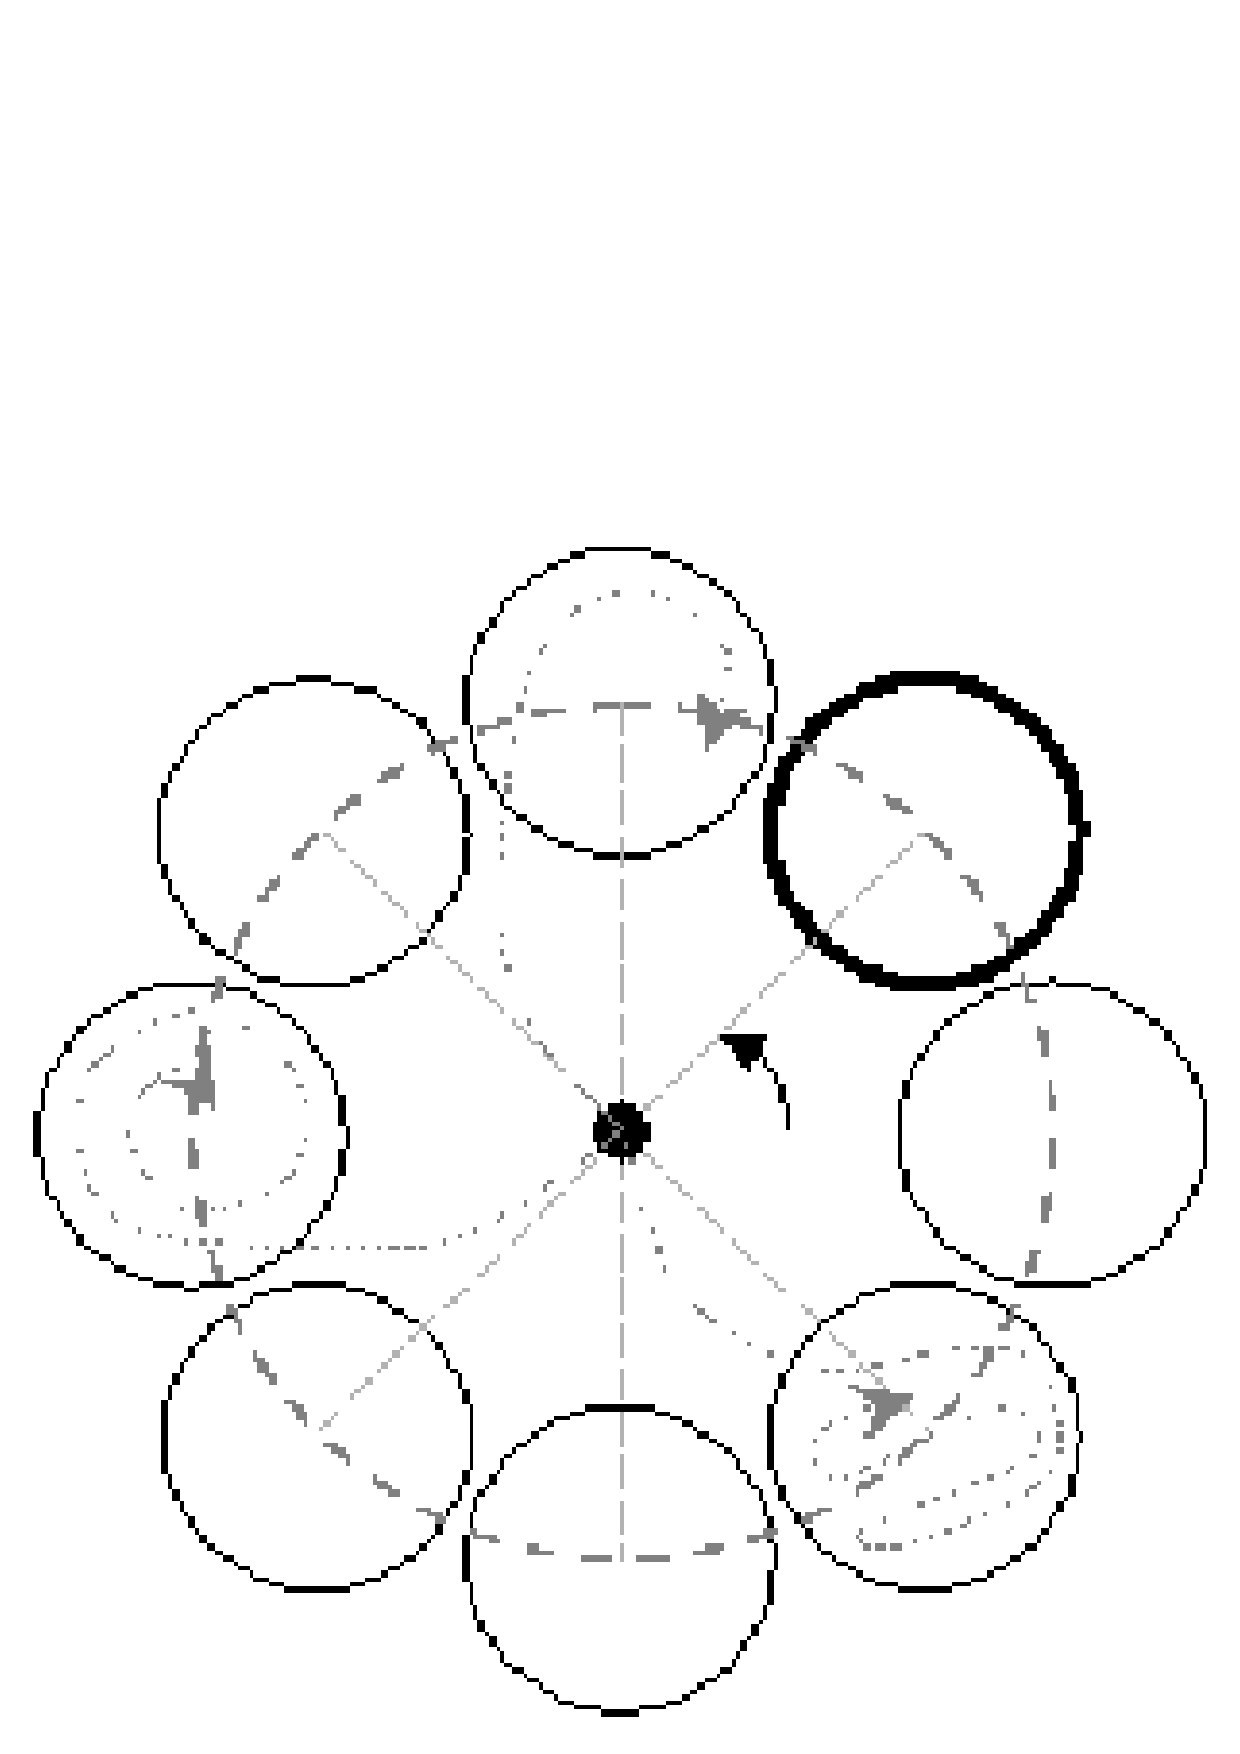
\includegraphics[width=.4\textwidth]{CloudSearch-1}
          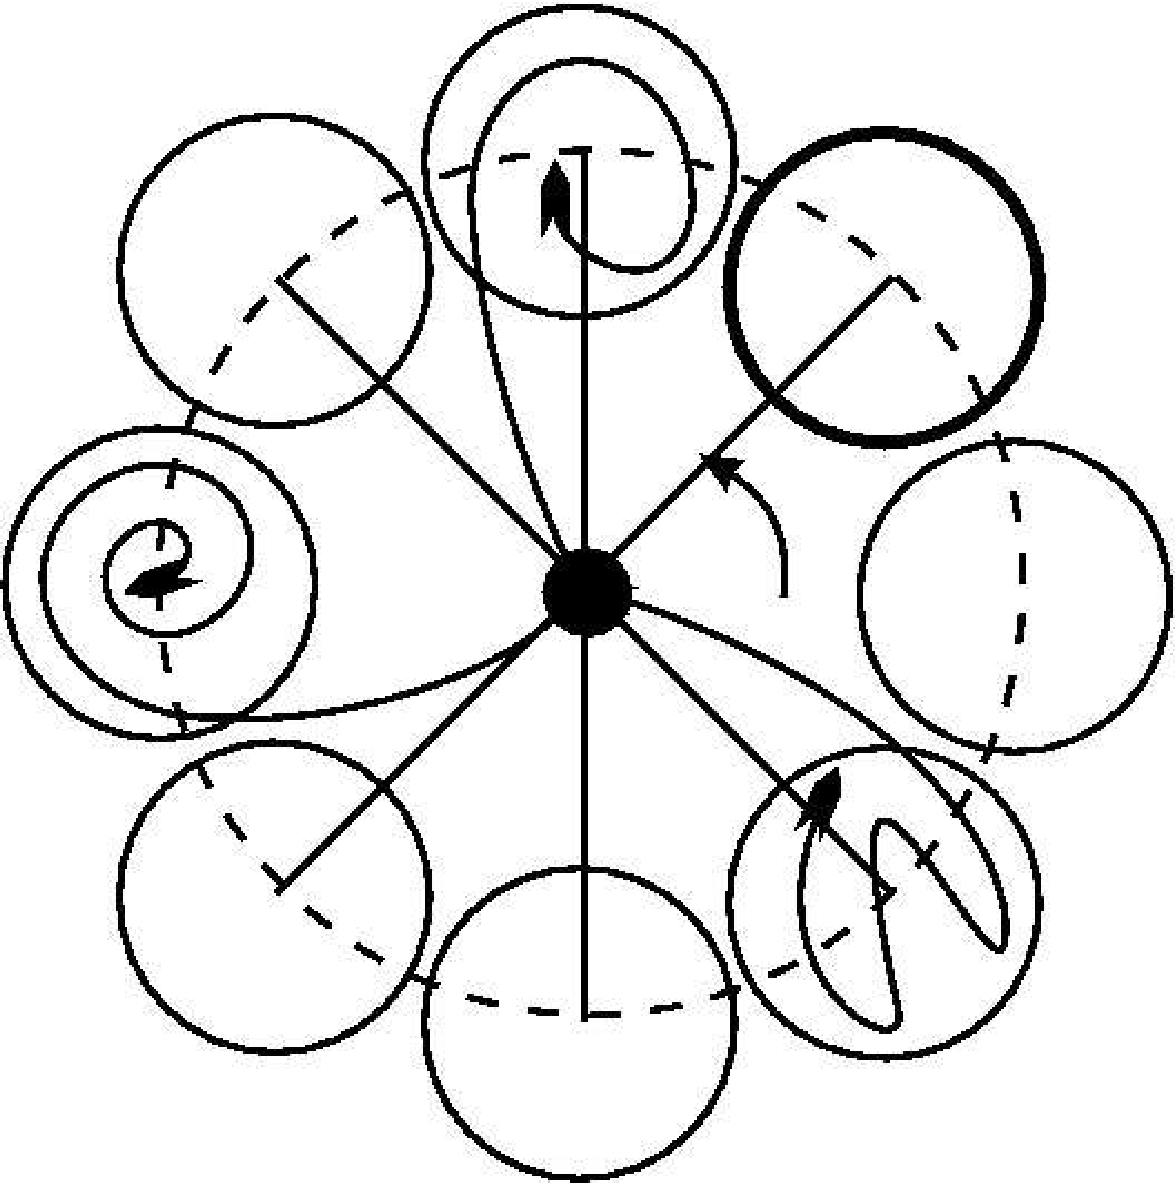
\includegraphics[width=.4\textwidth]{Radially_Symmetrical_Search}
	      \label{fig:SymmetricSearch-1}
	    } 
  \qquad
  \subfigure[Grid Symmetrical Search]
	    {
	      %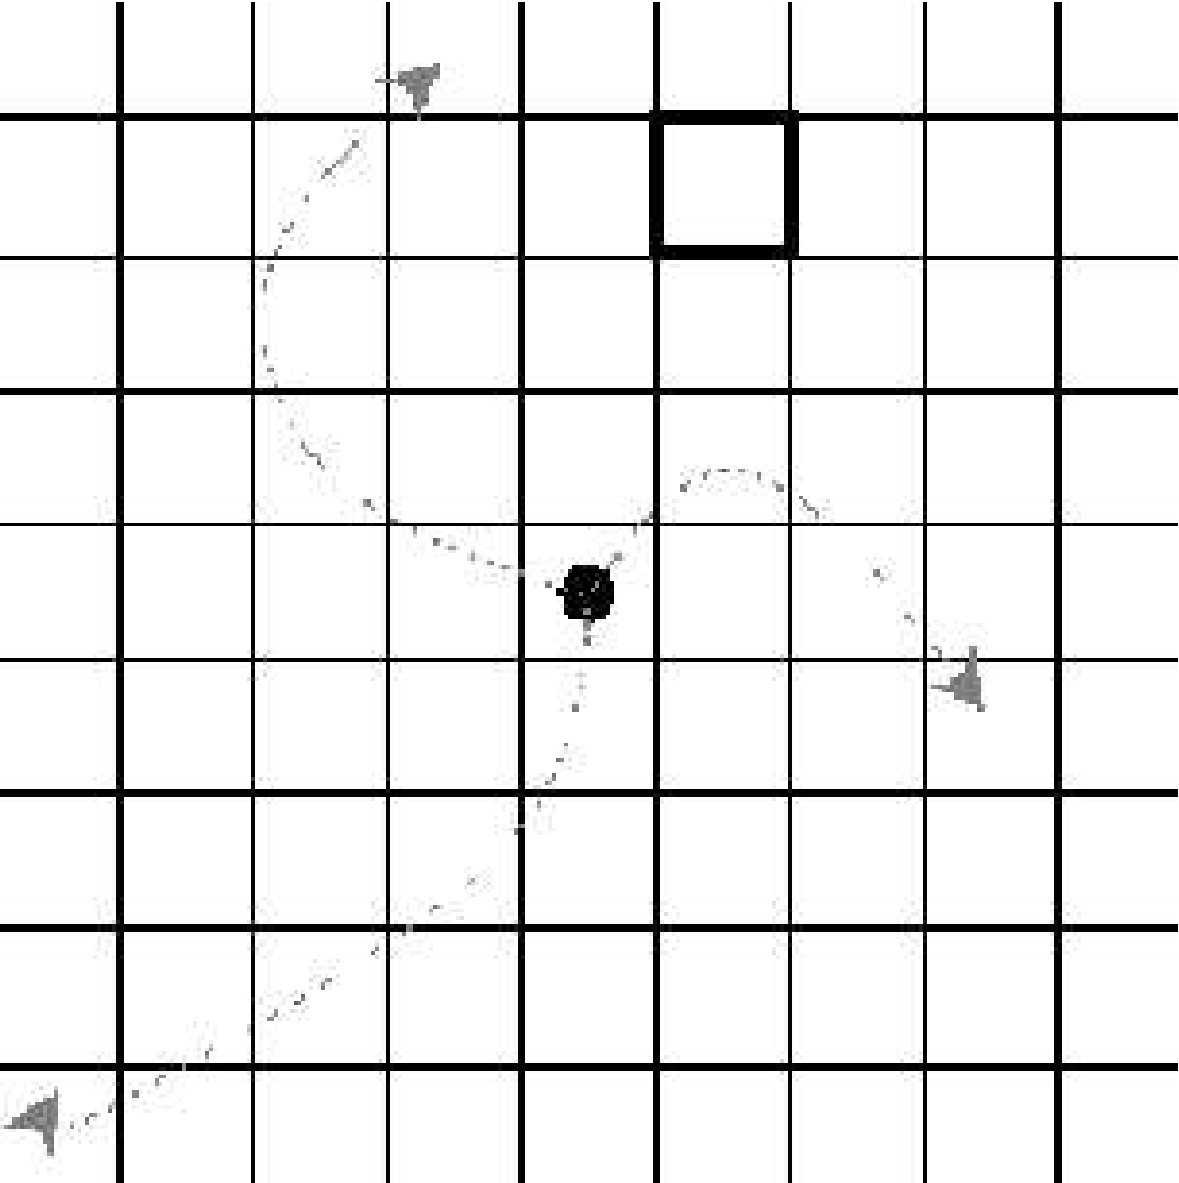
\includegraphics[width=.4\textwidth]{CloudSearch-2}
          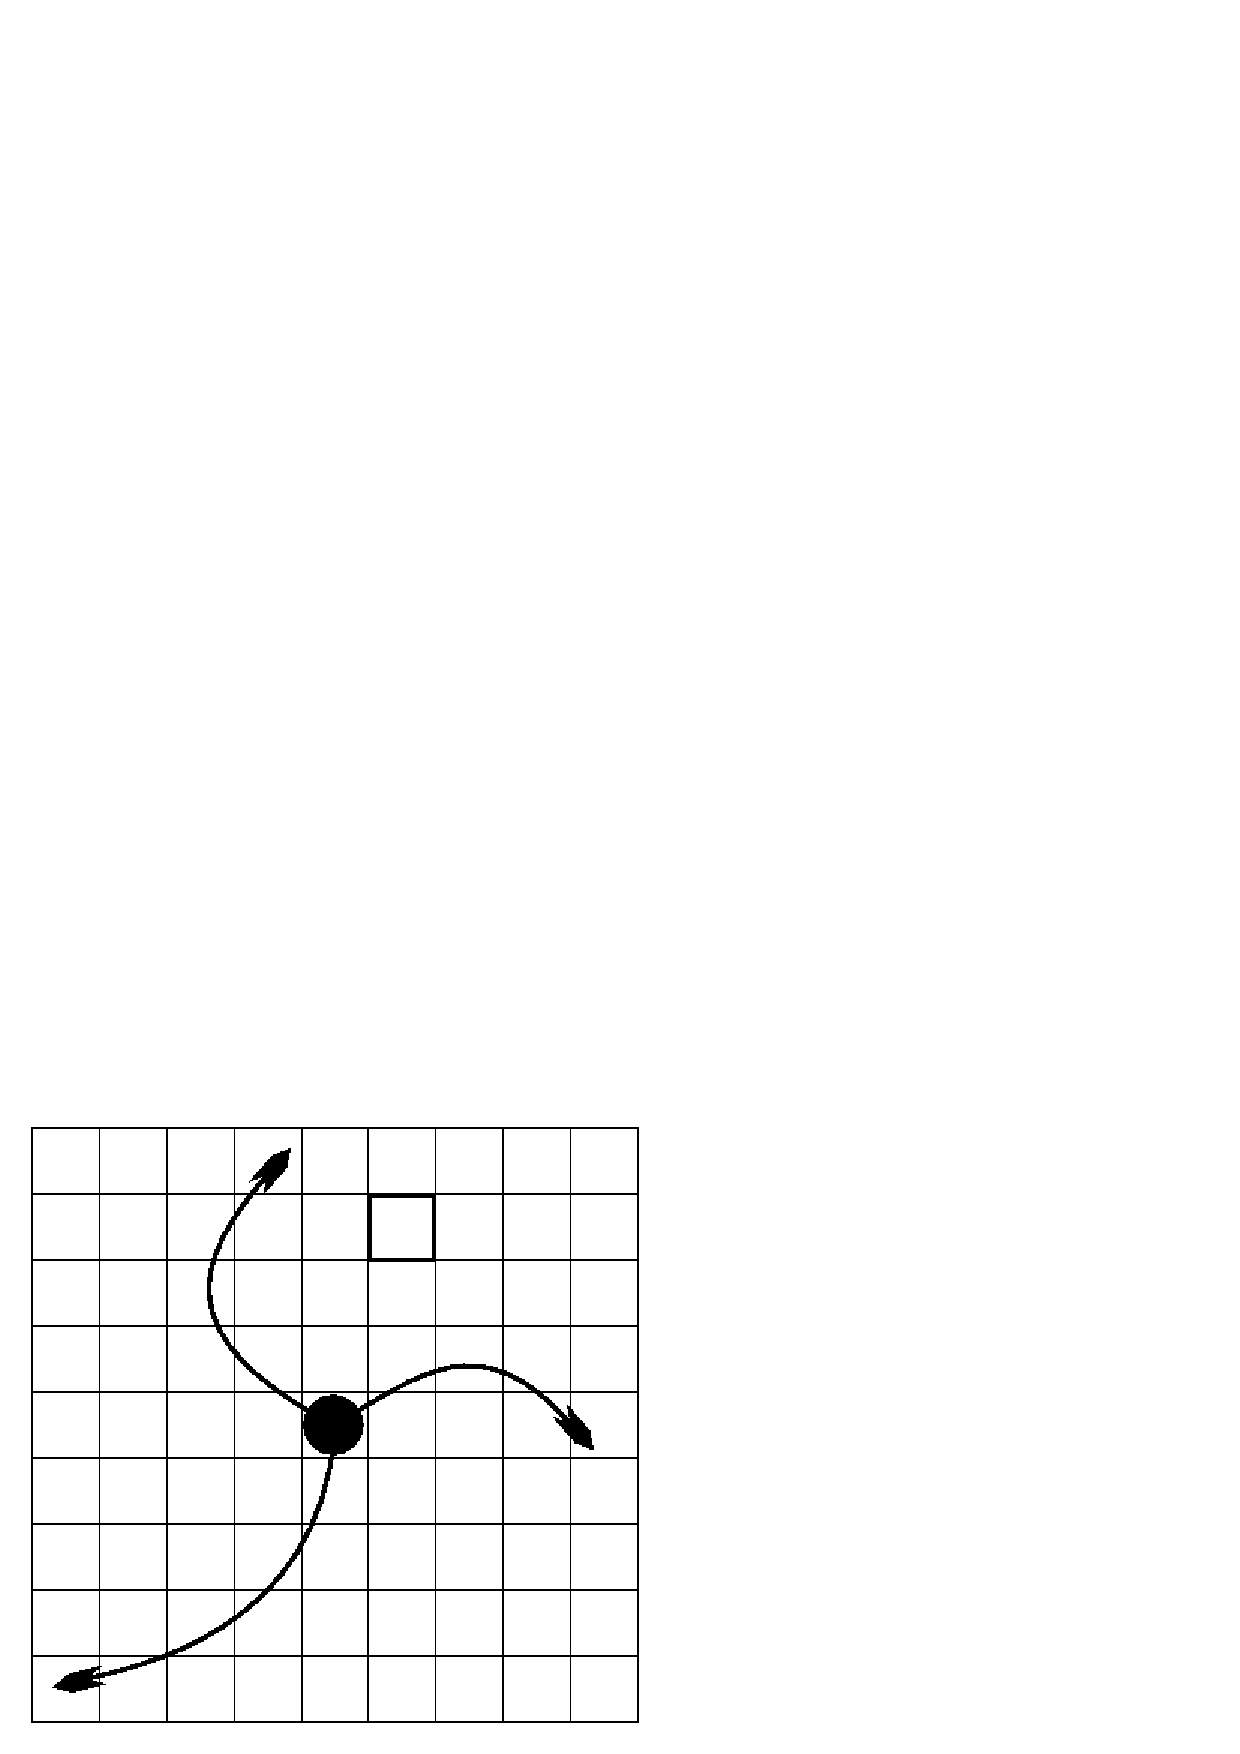
\includegraphics[width=.39\textwidth]{Grid_Symmetrical_Search}
	      \label{fig:SymmetricSearch-2}
	    }
	\quad
\caption[Examples of symmetrical search algorithms for UAVs.]{Examples of symmetrical search algorithms for UAVs.  In \refFigure{SymmetricSearch-1}, the symmetric subregions form a defense perimeter around a central point.  This strategy assumes that the area within the perimeter is clear and that the threat is coming from outside the perimeter.  In \refFigure{SymmetricSearch-2}, it is assumed the threat can be anywhere, thus each UAV is responsible for a set of subregions.}
\label{fig:SearchAlgorithms}
\end{figure}

\subsection{Cloud Detection and Mapping}

\paragraph{UAV Restrictions\\} The chemical cloud scenario imposes many restrictions on UAV swarms~\cite{clough:PersonalCommunication}. Generally, UAVs are capable of flying at speeds much greater than the average wind speed, thus causing a problem in cloud mapping because a UAV can easily out pace the cloud. The clouds involved in this scenario generally range from $\raise.5ex\hbox{$\scriptstyle 1$}\kern-.1em/ \kern-.15em\lower.25ex\hbox{$\scriptstyle 2$} $ km to 3 km in length. The cloud is relatively small as compared to the 10 km$^{2}$ region that must be patrolled. Since our swarms only consisted of 5 to 15 UAVs, detecting clouds of this size reliably made this scenario a good driving problem. Battery life was the largest restriction on the UAVs' capabilities. The UAVs evaluated had $\raise.5ex\hbox{$\scriptstyle 1$}\kern-.1em/ \kern-.15em\lower.25ex\hbox{$\scriptstyle 2$} $ hour of operational time, thus making it critical to manage flight time with respect to returning to base or a decontamination center.  Additionally, each UAV was equipped with a chemical sensor that possessed a 10 second processing latency.

Various enhancements to the UAV control schemes and search patterns arose from the restrictions placed upon the scenario. In order to improve the chances that a UAV swarm will successfully detect a chemical cloud, different search strategies were considered with the modification that UAVs would search in manners that \italic{cross-cut} the wind, \ie{} flying perpendicular to the wind direction.  For example, the symmetric sub-region search would have each UAV search their sub-region using this kind of \italic{cross-cutting}\footnote{Cross-cutting is defined as flying perpendicular to the wind direction.} pattern, shown in \refFigure{SymmetricSearch-1}. The random search strategy would have each UAV fly, and then at a randomly chosen moment cross-cut the wind for a time, then continue a random flight. An added bonus of cross-cutting the wind is that the UAVs can easily adjust to changing wind conditions by simply changing their cross-cutting vector.

\paragraph{Cloud Mapping\\} Once a chemical cloud is detected by the UAVs, its location and heading are known. By switching to alternative behavioral rules, the swarm can begin to ascertain the cloud's dimensions and density. With all types of mapping algorithms, the data collected must be adjusted with time to take into account for the movement and diffusion of the cloud. Either this can be done at a central location, or if capable, each UAV can manipulate the data itself. When considering algorithms for cloud mapping, the type of sensors that the UAVs are equipped with must be taken into account. Binary sensors, which deliver a \italic{chemical present/absent} signal, were assumed. There are two types of mapping strategies we considered: inside-outside and dispersion.

The inside-outside method is very straightforward, as illustrated in \refFigure{InOutlineMapping}. If an agent is inside a cloud, it chooses a direction and flies until it is outside of the cloud. Once outside of the cloud, the UAV chooses a point randomly offset from the last intersection with the cloud, and then flies back in. The points where the agent exits or enters the cloud, transition points, are then recorded. From this data, a model of the cloud size can be extrapolated.

\begin{figure}[ht]
  \centering
  \subfigure[Inside-outside mapping]
	    {
	      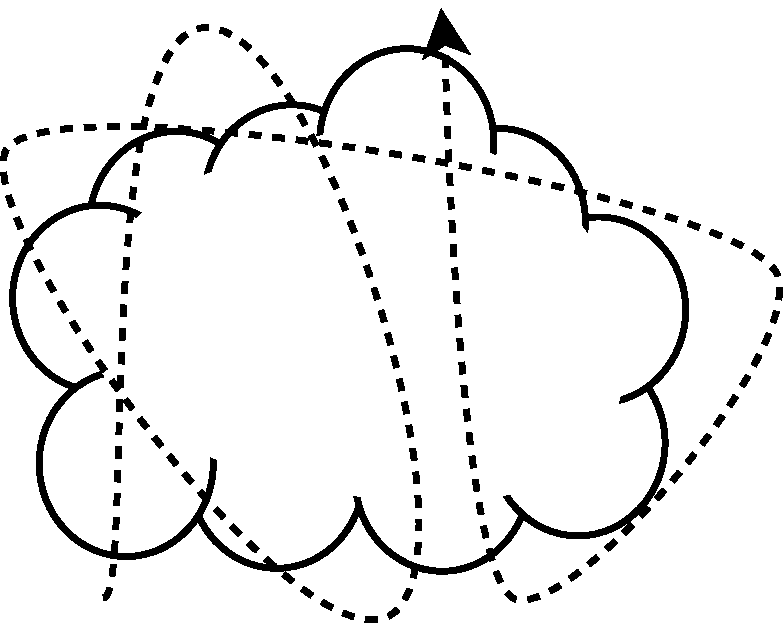
\includegraphics[scale=.35]{CloudMapping-InsideOutside}
	      %    \caption{The inside-outside cloud mapping behavior}
	      \label{fig:InOutlineMapping}
	    }
    \qquad
    \subfigure[Dispersion mapping]
	      {
		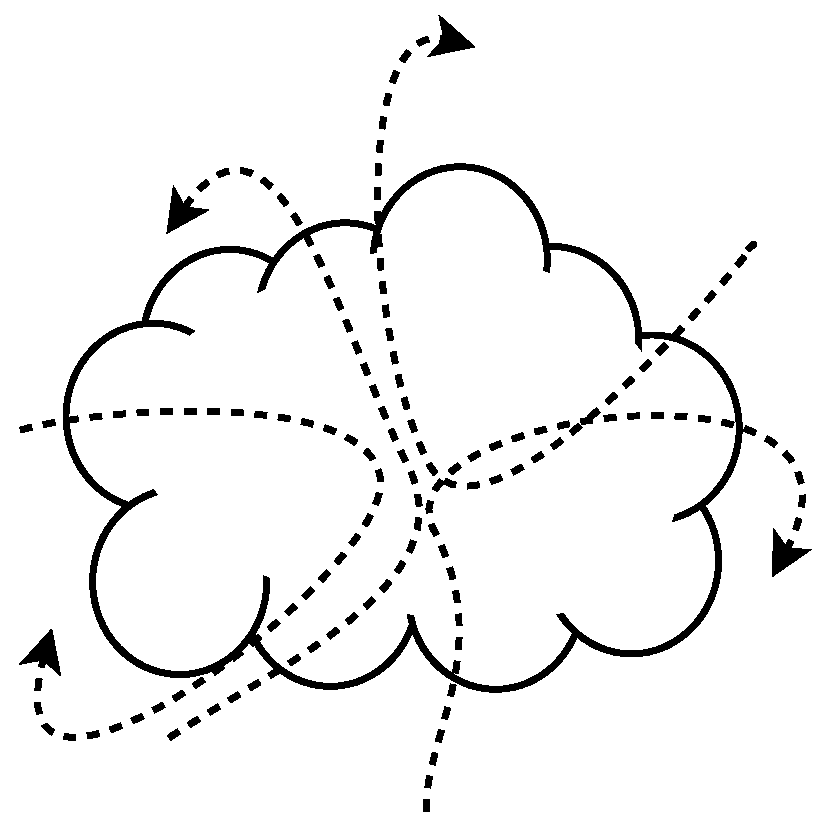
\includegraphics[scale=.35]{CloudMapping-Dispersion}
		%\caption{The dispersion cloud mapping behavior}
		\label{fig:DispersionMapping}
	      }
\caption{Examples of inside-outside and dispersion cloud mapping algorithms for UAVs}
\label{fig:MappingAlgorithms}
\end{figure}

A dispersion type algorithm can very effectively be used to map chemical clouds. Essentially, once a UAV detects the cloud, it broadcasts this information to all surrounding UAVs. After re-broadcasting the received message, the UAVs converge to the general area that the cloud was initially located and begin executing a dispersion algorithm. The agents execute the algorithm with only one modification; the UAVs continue to expand the dispersion area until a UAV is out of the cloud.  Thus, the boundary of the cloud is used as an additional constraint on the overall dispersion.  At this time, the UAVs outside the cloud begin moving back into the cloud, as seen in \refFigure{DispersionMapping}. Thus, the shape of the cloud emerges.

\subsection{Results}

\subsubsection{Chemical Cloud Mapping}

In order to demonstrate the capabilities of emergent behavioral strategies, a UAV rule-base was constructed for mapping a chemical cloud. The scenario used 10 UAVs in a bounded 10 km$^{2}$ region.  Each UAV had a 30 minute power supply, a maximum speed of 40 knots, and a sensor processing delay of 10 seconds.  The wind had a constant northeast direction at 4 knots.

Initially, a single UAV was placed in close proximity to the cloud while the rest of the UAVs were randomly distributed throughout the region, thus simulating an end-game situation for cloud searching. Quickly, a UAV finds the chemical cloud and broadcasts the location of the cloud. Upon receiving the broadcasts, the UAVs swarm to the general region where the cloud was found and begin the mapping process. For simulation purposes, the inside-outside mapping method, as previously described, was implemented. 

\refFigure{CloudMap} shows a plotting of the data the UAV swarm collected in approximately 15 minutes of flight time.  The white polygon represents the actual cloud.  The concentrations represent a post-processing of the data collected by the UAVs.  As can be clearly seen, the UAV swarm was able to determine the shape of the chemical cloud relatively quickly. The mapping of the cloud is an emergent behavior. In all three mapping strategies, no agent has any knowledge about the cloud's size, shape, or rate of diffusion. They simply randomly modify their behavior (change flight direction) whenever they detect an inside/outside transition. By recording the time and location of these transitions, the UAVs create a data set that contains all information necessary to accurately depict the cloud's movement over time. 

\begin{figure}[ht]
	\centering
	\vfill
	\begin{minipage}{\textwidth}
		\hfill
		\subfigure[Initial detection of the chemical cloud.]
		{
			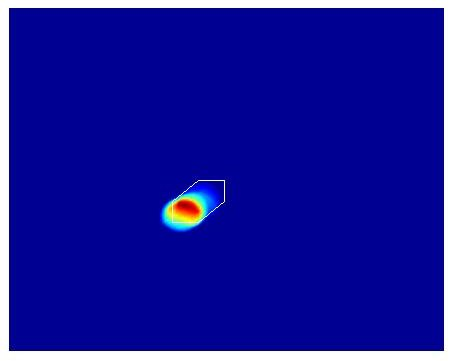
\includegraphics[width=.47\textwidth]{Figures/UAVmap1.jpg}
		}
		\hfill
		\subfigure[The cloud begins to slowly drift out of range.]
		{
			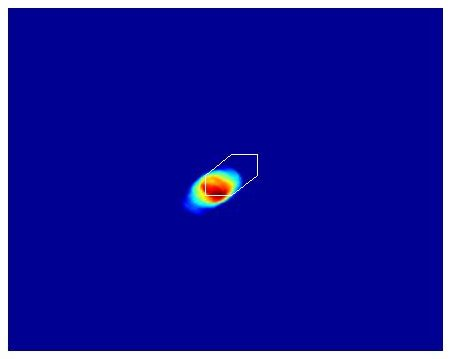
\includegraphics[width=.47\textwidth]{Figures/UAVmap2.jpg}
		}
		\hfill
	\end{minipage}
	\vfill
	\subfigure[The cloud is reacquired.]
	{
		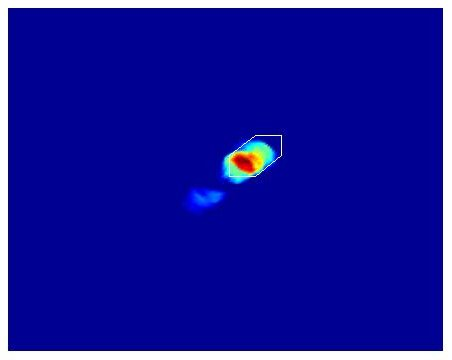
\includegraphics[width=.47\textwidth]{Figures/UAVmap3.jpg}
	}

\caption[Cloud mapping results for a swarm of 10 UAVs.]{Cloud mapping results for a swarm of 10 UAVs.  The white polygon represents the actual cloud.  The concentrations represent a post-processing of the data collected by the UAVs.}
\label{fig:CloudMap}
\end{figure}


\subsubsection{Chemical Cloud Searching Scenario}

The scenario chosen for the trade-off study was the detection of a chemical cloud by a UAV swarm. The purpose of this trade-off study is to empirically determine the best size for a UAV swarm searching a bounded region for a hostile-released chemical cloud. In this scenario, a UAV swarm is deployed from a central tower in a square region. Since the main objective of the swarm is detection of chemical clouds, it is unknown to the swarm whether there previously existed a chemical cloud in the region they patrol. Once released, the UAV swarm executes a search strategy in order to detect the presence of a chemical cloud. If the cloud is not found before the UAVs' power supplies are depleted, the swarm returns to the tower. When the chemical cloud is observed, the UAV swarm can transition into multiple cloud-mapping behaviors, which report sensor-based information such as cloud size, density, and composition. 

The swarm is responsible for patrolling a bounded square region. The intended target is a chemical cloud of unspecified size or type that moves with the wind. The chemical cloud is capable of diffusion, thus there is a fleeting window of time in which the cloud can be detected before the cloud has diffused completely. Also, the cloud diffusion causes the size of the cloud to increase, thus improving the chances of detection, while at the same time causing a decrease in cloud density. 

The UAV swarm used a modified random search to detect the cloud. Since the UAVs are capable of detecting wind direction, a wind cross-cutting addition was made to the randomized search. When en route to a randomly chosen destination, the UAV can decide to randomly cross-cut the wind, thus increasing the chances of finding the cloud. The UAV will cross-cut the wind for a random amount of time, then resume the randomized search.

Though there are more structured search algorithms, the nature of the scenario lends itself to the randomized search. As Clough states in \cite{clough:SwarmingUAVs}, \qw{random searches are optimal given no \apriori{} information.} Consider the case where the wind speed is 0 m/s, thus the cloud does not move and has minimal dispersion. In this case, more structured search algorithms will outperform the randomized search. Since the cloud does not move, a previously searched location need not be searched again. Thus, information does not become stale, and the swarm can systematically search the region with confidence. In more reasonable cases, the wind is driving a cloud along a path, and since the UAV swarm has no \apriori{} knowledge about the cloud's location, information is only fresh for a wind-speed dependent amount of time.  
%Since the UAV swarms being considered are relatively small (typically between 5-15 agents) and more complex algorithms provided no additional benefit, the trade-off study only examined the performance of the randomized search algorithm.

We examined cases of the chemical cloud scenario with UAV swarms of sizes 5 through 15 in a region that measured 10,000 m$^{2}$. Cloud size varied from 1 km to 3 km in length, and 1 km to 1.5 km in width. The size of the cloud was regulated using diffusion and decay parameters. The cloud was simulated as if there existed a single moving source of the chemical (\eg{} a crop duster).

The cloud lengths, beginning at 1 km, were incremented by 0.1 km. For each cloud length, 100 simulations were executed for each discrete swarm size, starting at 5 and incrementing up to 15, for a total of 30,000 simulations. The simulations ran until either the cloud was detected or the swarm ran out of fuel. The time to cloud detection was recorded and presented in \refFigures{Results-a}{Results-d}.

As the figures indicate, there is a performance increase when the number of agents is increased for the same-sized cloud. \refFigure{Results-a} represents the normalized amount of time taken by a UAV swarm to locate a chemical cloud. The search times were normalized against the total amount of time with which the UAV swarm could have searched. As expected, larger swarms were able to find similarly sized chemical clouds faster than smaller sized swarms.

\refFigure{Results-b} represents the percentage of times that the UAV swarm was able to successfully detect the chemical cloud. An increase in the number of UAVs in the swarm increases the swarm's chances of finding the chemical cloud because probabilistically speaking, more of the territory is being covered. 

\refFigure{Results-c} illustrates the average hit percentage of a UAV swarm of size $n$ for any sized cloud. \refFigure{Results-d} represents the average amount of time taken by a UAV swarm of size $n$ to find any sized cloud. As can be seen, even with the maximum number of agents, the chances of a UAV swarm finding a cloud of indeterminate size is 83{\%}. This performance rating may be acceptable for some situations, for example, if the UAV swarm is used as an early detection system. As shown in \refFigure{Results-c} and \refFigure{Results-d}, there exists a linear improvement in the performance of the UAV swarm with the addition of each agent. 

\clearpage

%\begin{figure}[ht]
%	\centering
%  	\fbox{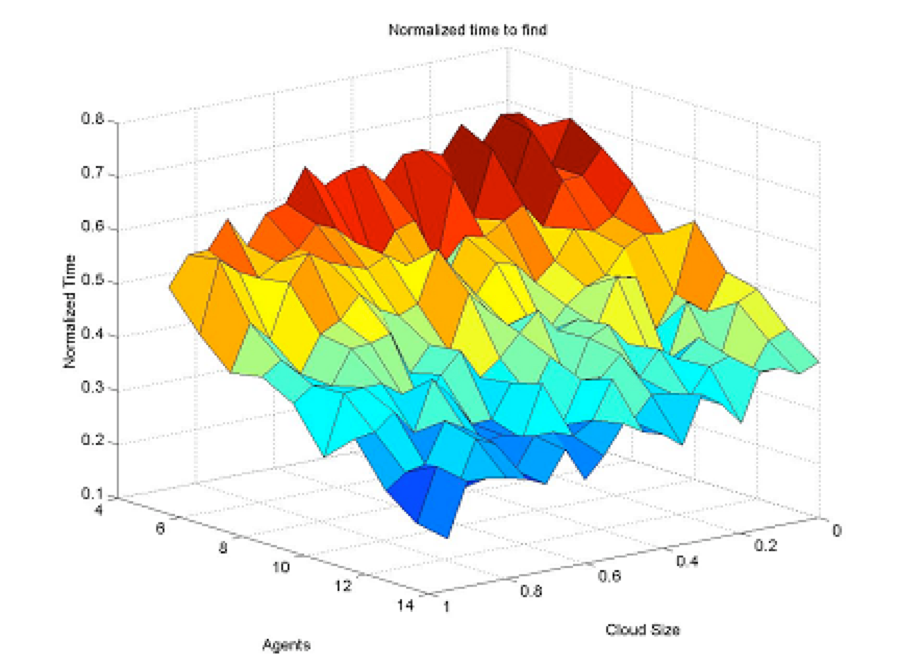
\includegraphics[scale=.6]{Figures/CloudTracking_Time.pdf}}
%\caption{This figure shows the normalized amount of time taken by a UAV swarm to locate a chemical cloud.  As expected, larger swarms were able to find similarly sized chemical clouds faster than smaller sized swarms.}
%\label{fig:Results-a}
%\end{figure}

%\begin{figure}[ht]
%	\centering
%  	\fbox{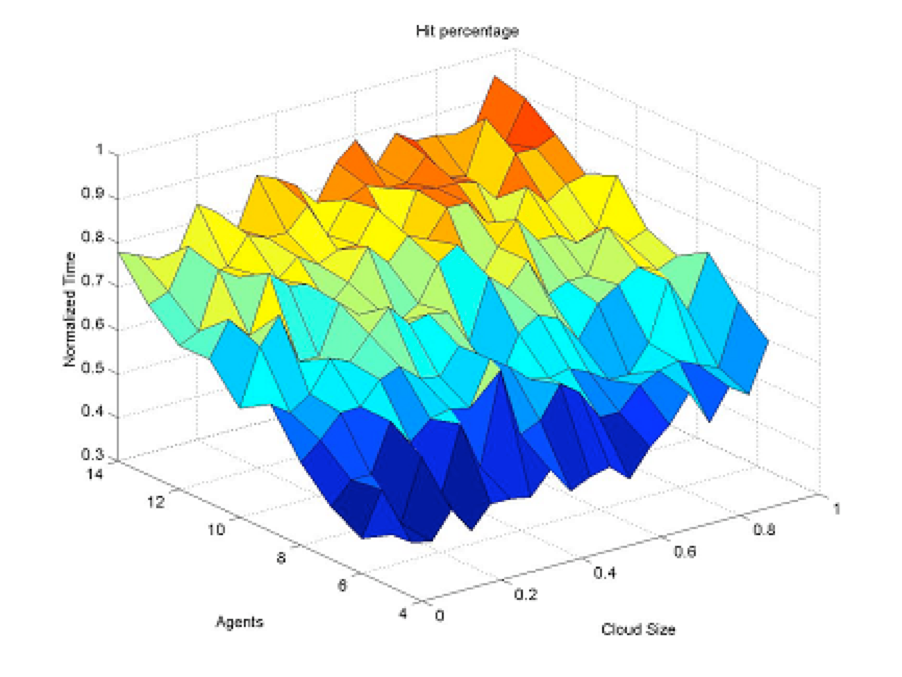
\includegraphics[scale=.6]{Figures/CloudTracking_Success.pdf}}
%\caption{This figure shows the percentage of times that the UAV swarm was able to successfully detect the chemical cloud.  An increase in the number of UAVs in the swarm increases the swarm's chances of finding the chemical cloud because more of territory is being covered.}
%\label{fig:Results-b}
%\end{figure}

\begin{figure}[ht]
	\centering
	\vfill
  	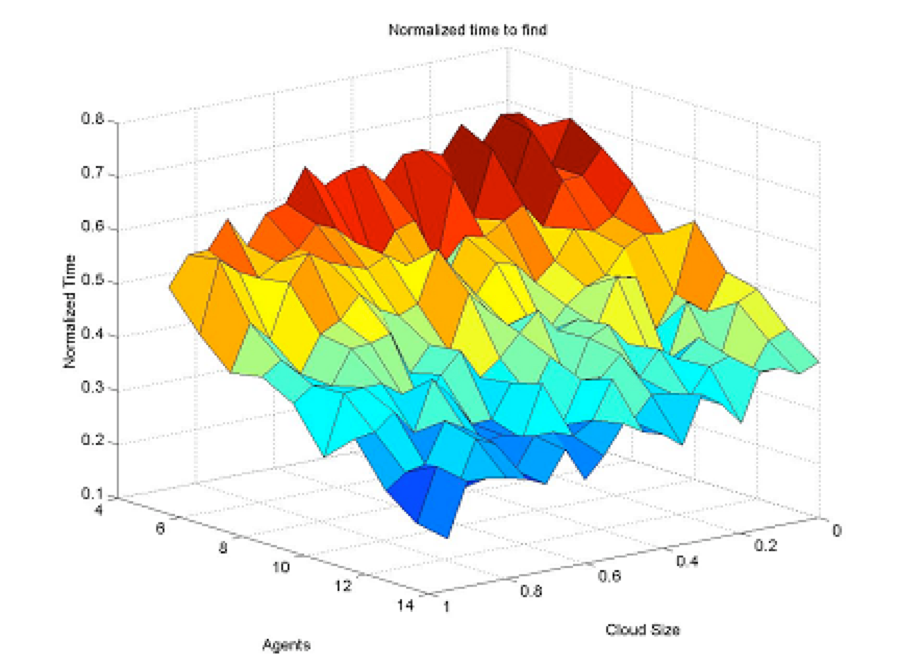
\includegraphics[scale=.75]{Figures/CloudTracking_Time.pdf}
\caption[The normalized amount of time taken by a UAV swarm to locate a chemical cloud.]{This figure shows the normalized amount of time taken by a UAV swarm to locate a chemical cloud.  As expected, larger swarms were able to find similarly sized chemical clouds faster than smaller sized swarms.}
\label{fig:Results-a}
	\vfill
	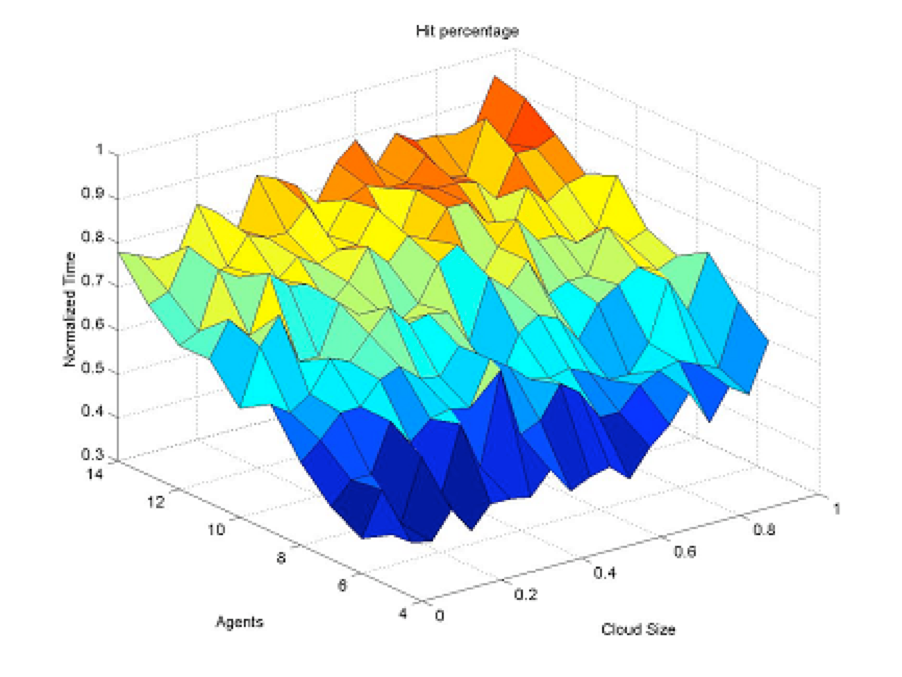
\includegraphics[scale=.45]{Figures/CloudTracking_Success.pdf}
\caption[The percentage of trials where the UAV swarm successfully detects the chemical cloud.]{This figure shows the percentage of trials in which the UAV swarm was able to successfully detect the chemical cloud.  An increase in the number of UAVs in the swarm increases the swarm's chances of finding the chemical cloud because more of the territory is being covered.}
\label{fig:Results-b}
	\vfill
\end{figure}

\begin{figure}[ht]
	\centering
   	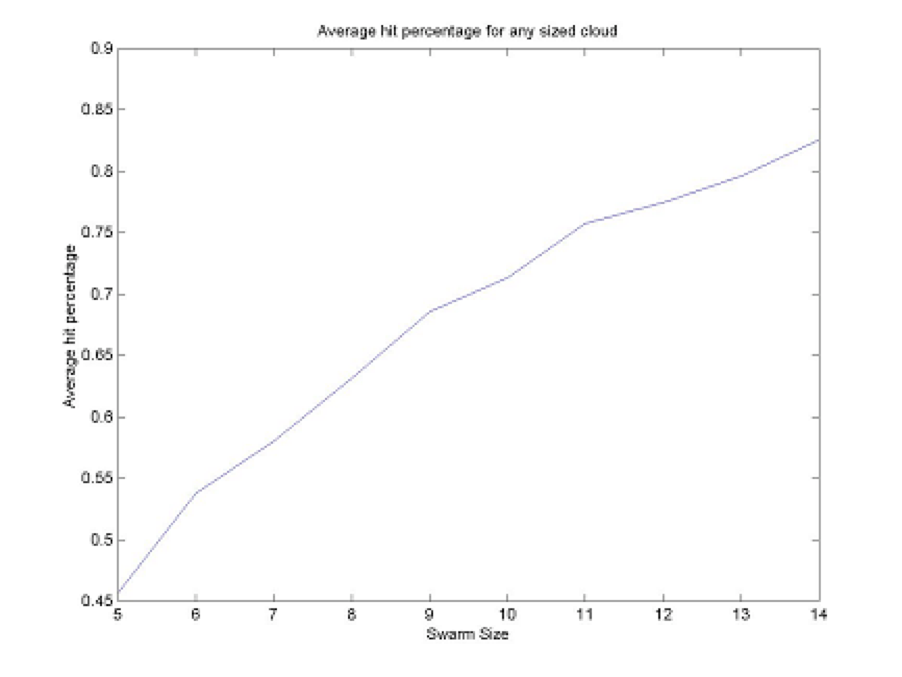
\includegraphics[scale=.75]{Figures/CloudTracking_HitPercentage.pdf}
\caption[The average hit percentage of a UAV swarm of size $n$ for any sized cloud.]{This figure shows the average hit percentage of a UAV swarm of size $n$ for any sized cloud.  With the maximum number of agents, the chances of a UAV swarm finding a cloud of indeterminate size is 83\%.}
\label{fig:Results-c}
%\end{figure}
%\begin{figure}[ht]
%	\centering
   	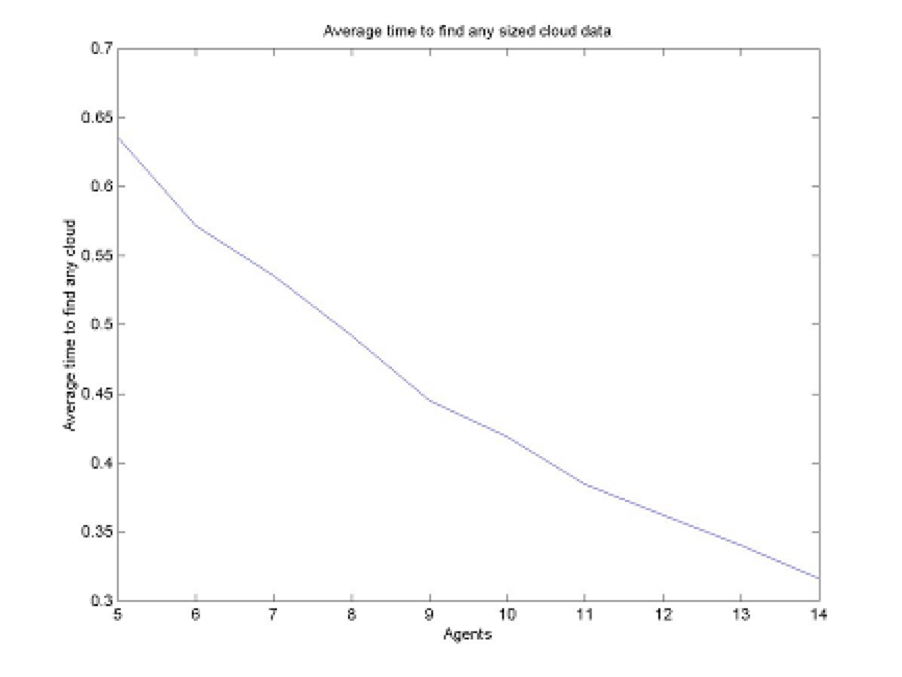
\includegraphics[scale=.75]{Figures/CloudTracking_AverageTime.pdf}
\caption[The average amount of time taken by a UAV swarm of size $n$ to find any sized cloud.]{This figure shows the average amount of time taken by a UAV swarm of size $n$ to find any sized cloud.  Notice that there exists a linear improvement in the performance of the UAV swarm with the addition of each agent.}
\label{fig:Results-d}
\end{figure}
